


%\section{Tecnologías utilizadas}

%Para el desarrollo del proyecto he usado el lenguaje de programación \textbf{python}, con el IDE PyCharm. La librería principal, bajo la que se sustenta el servidor es \textit{web.py}. Alternativas a esta librería pueden ser Flask o Django. Sin embargo esta última es para proyectos mucho más grandes. La ventaja de web.py es lo ligera qué es y la facilidad de ponerla en marcha.
%Otra librería muy utilizada ha sido requests, para realizar peticiones HTTP tanto a la API Hubspot como el envio de mensajes Soap a los servicios web de Workday.
%Para la prueba de los mensajes Soap, he utilizado la herramienta SoapUI.

%También he hecho uso de la paquete \textbf{lxml} para la creación de árboles \textbf{\acrshort{xml}} y la transformaciones \acrshort{xslt}.

%Internamente he usado como base de datos SQLite3 para python. En esta base de datos se almacena la correspondencia entre los deals de HubSpot y los proyectos de Workday.

%Para el uso de los servicios web de Workday, se mandan mensajes \acrshort{soap} por HTTP.



\chapter{Integración}

Para poder entender la Interfaz que he desarrollado debemos poder observar el contexto en el que se encuentra. En la figura \ref{fig:general_diagram} podemos ver cada aplicación y las relaciones de comunicación que existen entre ellas.\\

\begin{figure}[H]
\centering

    
\pagestyle{empty}
\begin{tikzpicture}
  \path[mindmap,concept color=black,text=white]
    node[concept] {\Large \textbf{Interfaz}}
    [clockwise from=120]
    child[concept color=orange, text=black] {
      node[concept] {App HubSpot}
      [clockwise from=90, inner sep=0.1cm]
      child { node[concept] {\textbf{HubSpot}} }
    }
	child[concept color=blue!35!cyan, text=black] {
      node[concept] {\textbf{Workday}}
    }
    ;
\end{tikzpicture}



\caption{Diagrama general del sistema \protect\footnotemark{}} 
\label{fig:general_diagram}
\end{figure}

\footnotetext{Modificación del ejemplo de \href{http://www.texample.net/tikz/examples/computer-science-mindmap/}{\textit{Till Tantau}}}	

La Interfaz esta conectada tanto a HubSpot como a Workday. A HubSpot se conecta a través de una aplicación que hay que crear en HubSpot y la comunicación  puede ser bidireccional. De la \textit{Interfaz} hacia Hubspot se hace mediante peticiones \acrshort{http} a la \acrshort{api} de Hubspot. La otra comunicación en la otra dirección se realiza mediante los webhooks declarados en la aplicación de Hubspot.\\

Sin embargo en Workday la comunicación es unidireccional, únicamente de la Interfaz hacia Workday. Workday sí que responde a algunas peticiones \acrshort{http} con información, pero nunca inicia un mensaje hacia la Interfaz.

\section{HubSpot}
En esta sección vamos a describir toda la información que necesitamos saber sobre HubSpot para entender la \textit{Interfaz}.

Hubspot se encuentra organizado en objetos y cada objeto tiene un conjunto de propiedades.
En Hubspot existen múltiples objetos, pero los objetos que nos interesan para nuestra integración son \textit{deal} y \textit{company}


En HubSpot un deal puede estar asociado a una o más \textit{companies}. Para el caso de nuestra integración a lo sumo habrá un \textit{company} asociado a cada \textit{deal}.

\subsection{Deal}
	Es un objeto de Hubspot que representa una oportunidad de negocio con cierto cliente. Por defecto en Hubspot tenemos las siguientes propiedades asociadas a un deal:			
		Deal Id, Amount, Close Date, Closed Lost Reason, Closed Won Reason, Create Date, Deal Description, Deal Name, Deal Stage, Deal Type, HubSpot Owner, Last Activity Date, Last Modified Date, Number of Contacts
		,Opp number,Owner Assigned Date, Pipeline y las personalizadas de la empresa: Practice, Transaction Amount, Transaction Currency
		
		Las propiedades más importantes a tener en cuenta en la integración son las siguientes:
		\begin{itemize}
			\item \textbf{Deal id}: Identificador unívoco del \textit{deal} de HubSpot.
			\item \textbf{Close date}: Se trata de la fecha en la que se ha cerrado el acuerdo.
			\item \textbf{Deal Description}: Información describiendo el \textit{deal}.
			\item \textbf{Deal name}: Nombre del \textit{deal}.
			\item \textbf{Deal Stage}: estado en el que se encuentra el \textit{deal}. Esta se trata de una de las propiedades más importantes. 
				Esta propiedad puede tomar los siguientes valores.
				\begin{itemize}
					\item[$\circ$] Appointment Scheduled: Cuando se ha fijado una cita con el cliente.
					\item[$\circ$] Initial Contact: Si ya se ha tenido un primer contacto con el cliente.
					\item[$\circ$] Opportunity Identfied: En caso de que se haya identificado una oportunidad de negocio con el cliente.
					\item[$\circ$] Preparing Proporsal: Si se está preparando una proposición de oferta al cliente.
					\item[$\circ$] Proporsal Sent: Una vez se haya enviado la proposición de oferta al cliente.
					\item[$\circ$] Decision Maker Bought In: Una vez la oferta ya esta hecha y el cliente tiene la posibilidad de decidir si la acepta o no.
					\item[$\circ$] Contract Sent: Cuando el contrato se ha enviado al cliente.
					\item[$\circ$] Closed Won: Si la oportunidad de negocio se ha cerrado favorablemente.
					\item[$\circ$] Closed Lost: En caso de que se haya perdido la oportunidad con el cliente.
				\end{itemize}
		\end{itemize}
		
		
		Es de especial importancia la propiedad \textit{Deal Stage}, ya que dependiendo de su valor se realizará o no la sincronización.
		La propiedad \textit{Deal Stage} representa el estado en el que se encuentra un \textit{deal}. Un \textit{deal} se clasifica en las siguientes fases:
		\begin{enumerate}
			\item \textbf{Fase de descubrimiento}: Fase inicial del \textit{deal}. Cuando un \textit{deal} se encuentra en esta fase, no se sincroniza con Workday. La información del \textit{deal} solo reside en Hubspot.
			\item \textbf{Fase de progreso}: fase intermedia del proceso en la que todavía esta por decidir si la oportunidad se va a ganar o no. Todos los \textit{deals} en esta fase se mantienen sincronizados con el correspondiente proyecto de Workday.
			\item \textbf{Fase de cierre}: Fase final del proyecto. Una vez un \textit{deal} ha alcanzado esta fase, se excluye la oportunidad y no se continua sincronizando. Desde este momento se trata de manera independiente el proyecto en Workday, y el \textit{deal} no se modifica más. 
		\end{enumerate}
		
		\begin{figure}[H]
\centering
\begin{tikzpicture}[
	scale=0.75,
	start chain=1 going below, 
	node distance=1mm,
	stage/.style={
		scale=0.75,
		on chain=1,
		rectangle,
		rounded corners,
		draw=black, 
		very thick,
		text centered,
		text width=8cm,
		minimum height=12mm
		},
	discovery/.style={
		fill=cyan!30
	},
	progress/.style={
		fill=blue!30
	},
	closure/.style={
		fill=green!30
	},
	phase/.style={
		scale=0.75,
		on chain=1,
		minimum height=12mm,
		text width=2cm,
		text centered
	},
	every node/.style={font=\sffamily}
]



% Discovery phase
\node [stage, discovery] (AS) {Appointment Scheduled};
\node [stage, discovery, continue chain=going below] (IC) {Initial Contact};
% Progress phase
\node [stage, progress] (OI) {Opportunity Identfied};
\node [stage, progress] (PP) {Preparing Proporsal};
\node [stage, progress] (PS) {Proporsal Sent};
\node [stage, progress] (DM) {Decision Maker Bought In};
\node [stage, progress] (CS) {Contract Sent};
% Closure phase
\node [stage, closure] (CW) {Closed Won};
\node [stage, closure] (CL) {Closed Lost};

\draw [
    thick,
    decoration={
        brace,
        mirror,
        raise=0.5cm
    },
    decorate
](AS.west) -- (IC.west) node[midway,xshift=-2cm] {descubrimiento}; 

\draw [
    thick,
    decoration={
        brace,
        mirror,
        raise=0.5cm
    },
    decorate
](OI.west) -- (CS.west) node[midway,xshift=-2cm] {Progreso}; 


\draw [
    thick,
    decoration={
        brace,
        mirror,
        raise=0.5cm
    },
    decorate
](CW.west) -- (CL.west) node[midway,xshift=-2cm] {Cierre};

\end{tikzpicture}
\caption{Estados por los que pasa un deal \protect\footnotemark{}}
\label{fig:deal_phases}
\end{figure}



\footnotetext{Modificación del ejemplo de \href{http://www.texample.net/tikz/examples/pera-model/}{\textit{Erno Pentzin}}}	
		
		Todo \textit{deal} empieza con un estado perteneciente a la fase de descubrimiento, con el paso del tiempo puede ir pasando a la fase de progreso y finalmente todo deal termina en uno de los dos estados de la fase de cierre: \textit{Closed Won} y \textit{Closed Lost}.
			
			
			
		Además de propiedades, los objetos pueden tener asociaciones. En el caso del deal puede tener una o más \textit{companies} asociadas. La \textit{Interfaz}, dará por hecho que cada \textit{deal} está asociado a lo sumo a una \textit{company}.
			
		Desde el portal de HubSpot es posible tanto crear nuevos \textit{deals} como modificar cualquier propiedad (con excepción del Deal Id) o asociación de los \textit{deals} ya existentes.
		
		\begin{figure}
			\centering
			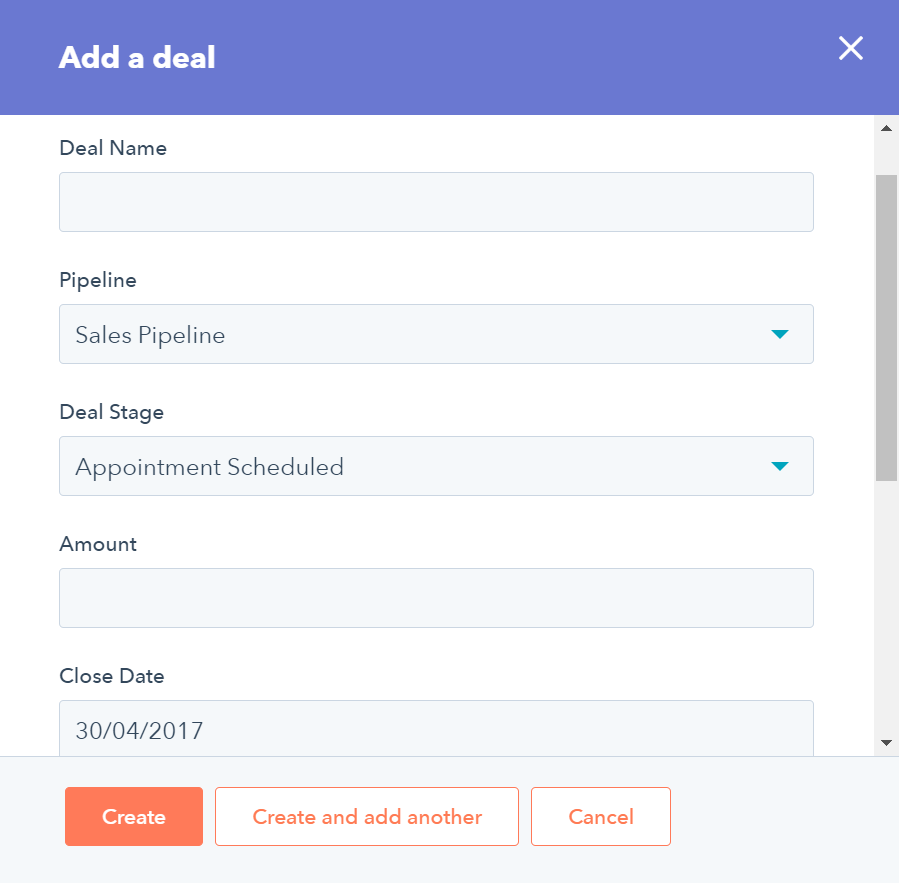
\includegraphics[width=0.5\textwidth]{deal_creation.png}
			\caption{Creando un deal desde el portal de HubSpot}
		\end{figure}

\subsection{Company}
		
		Es un objeto de HubSpot que representa una empresa. Este objeto cuenta con multitud de propiedades, que describen información de la empres, como puede ser información de contacto, localización \ldots 
		
		Desde el portal de HubSpot es posible tanto crear nuevas companies como modificar cualquiera de los ya existentes.
		
		\begin{figure}
			\centering
			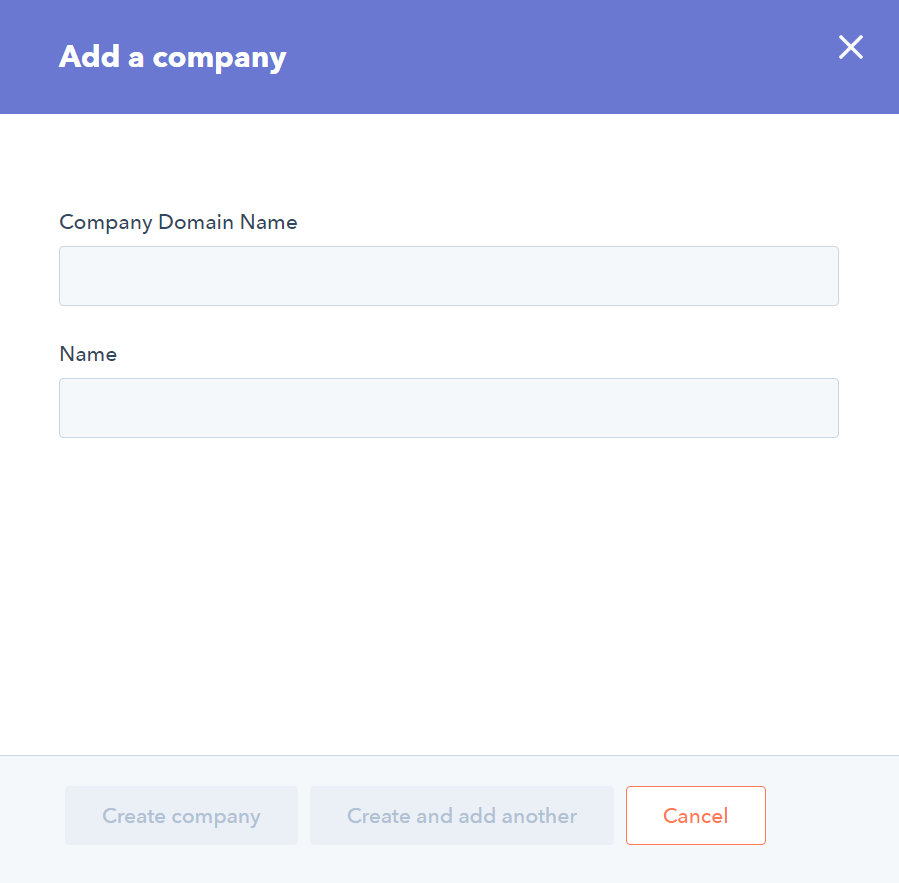
\includegraphics[width=0.5\textwidth]{company_creation.png}
			\caption{Creando una company desde el portal de HubSpot}
		\end{figure}


\subsection{Aplicación de Hubspot}
\label{subsec:app_hs}
Para poder realizar la integración y hacer uso de la \acrshort{api} de HubSpot \cite{hsapi}, es necesario crearse una cuenta de desarrollador. Con la cuenta de desarrollador podemos crear una aplicación y acceder a su panel de control. 
Desde el panel de control de la aplicación tendremos acceso a información importante para la integración, como son las claves (\verb|Client ID|, \verb|Client secret|).


También desde el panel de control de la aplicación deberemos especificar debemos indicar la dirección a la que deseamos que nuestros mensajes sean enviados y especificar los eventos de HubSpot ante los que se debe enviar un mensaje
En el caso de nuestra aplicación está suscrita a los siguientes eventos:

\begin{itemize}
	\item \textbf{deal.creation}: Cuando un nuevo deal es creado en HubSpot se envía un mensaje.
	\item \textbf{deal.propertyChanged} 
		\begin{itemize}
			\item \verb|dealstage|: Cuando en un deal de HubSpot se modifica el estado.
			\item \verb|practice|: Cuando en un deal de HubSpot se modifica la práctica.
			\item \verb|hubspot_owner_id|: Cuando en un deal de HubSpot se modifica su propietario.
			\item \verb|closedate|: Cuando en un deal de HubSpot se modifica la fecha de cierre.
			\item \verb|description|: Cuando en un deal de Hubspot se modifica la descripción.
			\item \verb|dealname|: Cuando en un deal de Hubspot se modifica el nombre.
			\item \verb|transaction_currency|: Cuando en un deal de HubSpot se modifica la moneda.
			\item \verb|legal_entity|: Cuando en un deal de HubSpot se modifica la entidad.
		\end{itemize}
\end{itemize}

Desde el panel de control de la aplicación de HubSpot también tenemos acceso a las claves (\verb|Client ID|, \verb|Client secret|) para poder instalar la aplicación en tantos portales como deseemos. En nuestro caso solo será uno.


Para instalar una aplicación en un portal de HubSpot hay que seguir un proceso de autorización llamado \gls{oauth2} que ha sido automatizado he integrado en la interfaz creada. 
Los pasos que hay que seguir son los siguientes \cite{hsapi}:
%TODO diagram oauth2

\begin{enumerate}
	\item Dirigirse a la url \url{https://app.hubspot.com/oauth/authorize?client_id=<client_id>&scope=contacts&redirect_uri=https://www.hubspot.com/}
		\\ 
		sustituyendo \textless client\_id\textgreater por el su valor. Y autorizar la instalación de la aplicación. Cabe destacar que solo se puede acceder a dicha url  y por tanto instalar la aplicación si se cuenta con el \verb|Client ID|.
		Haciendo público el \verb|Client ID| de la aplicación , esta puede ser instalada por cualquier persona. En nuestro caso este valor permanecerá en privado y solo nosotros haremos uso de la aplicación.
		
	\item Tras dar acceso al portal se te redirige a una página en la que aparece un código concatenado a la url.
	\item Mediante este código, el \verb|Client ID| y el \verb|Client secret| podemos obtener un token de sesión.
	Tras hacer la petición a la API de HubSpot, nos devolverá un mensaje con los siguientes valores.
		\begin{itemize}
			\item \verb|access_token| clave usado para realizar las peticiones a la API de HubSpot.
			\item \verb|refresh_token| usado para conseguir nuevo par (\verb|access_token|, \verb|refresh_token|) cuando el \verb|access_token| ha expirado.
			\item \verb|expires_in| tiempo en milisegundos de validez del \verb|access_token|.
		\end{itemize}
	\item Cuando el \verb|access_token| haya expirado podremos llamar a otro endpoint especificando el \verb|refresh_token| y recibiremos un mensaje de vuelta con otro nuevo \verb|access_token| y \verb|refresh_token|.
\end{enumerate}



\section{Workday}

En esta sección vamos a describir la información que necesitamos saber sobre Workday.

Workday es un ERP que internamente se encuentra organizado en objetos. Los objetos que van a ser de interés para realizar la integración son:
Project, Customer y Hierarchy.

Además cada uno de estos objetos cuenta con una serie de campos, que pueden incluso hacer referencia a otros objetos.


Para realizar las integraciones, Workday proporciona servicios web que están en constante actualización.
Mediante estos servicios podemos hacer que la Interfaz interactúe con Workday.



\subsection{Project}
Es un objeto de Workday y existe una instancia por cada proyecto. Dentro de nuestra integración, 
el objeto Project de Workday está relacionado con el objeto Deal de HubSpot. 
De forma que por lo general las acciones sobre el objeto Deal en HubSpot darán lugar a otros eventos
 sobre el objeto Project de Workday.
 
Un objeto Project puede ser creado de manera manual, pero en nuestra integración, esto se realizará mediante los servicios web.
Para crear o modificar un proyecto ya existente hay que enviar un mensaje SOAP por HTTP. 
Para ello hay que usar la operación \verb|Submit_Project|  incluida en el servicio \verb|Resource_Management|.

El objeto Project cuenta con multitud de campos: 

\begin{itemize}
\item Project name: Nombre del proyecto, está sincronizado con el nombre del deal correspondiente.
\item Start Date: Fecha de inicio, está sincronizado con con la propiedad \verb|close_date| del deal.
\item Status: Estado del proyecto, existe una correspondencia con la propiedad \verb|deal_stage| del deal en HubSpot.
\item Description: Descripción del proyecto. Este campo se encuentra sincronizado con la propiedad \verb|description| del deal.

%y campos que hacen referencia a otros objetos como son: 
\item Project Hierarchy: La Jerarquía principal del proyecto. Este campo está en directa relación con la propiedad personalizadas
\verb|practice| de HubSpot.
\item OptionalProject Hierarchy: La jerarquía opcional del proyecto. Este campo se encuentra directamente relacionado con la propiedad \verb|hubspot_owner_id| del correspondiente deal.
\item Customer: El cliente del proyecto. Existe una correspondencia entre el cliente y la asociación \verb|associated_company| del deal en HubSpot.

\end{itemize}



\subsection{Customer}
Se trata de un objeto de Workday que representa a los clientes de la empresa. este objeto de Workday se encuentra relacionado con el objeto company de Hubspot. 
Gracias a la Interfaz, cuando se realice la integración de un \textit{deal}, también se integrará la \textit{company} asociada.

Existen múltiples métodos para crear o modificar un \textit{Customer} en Workday, de forma manual, hojas de calculo para carga de datos \ldots

En nuestro caso la creación y modificación de un cliente se hace desde la Interfaz, 
mediante la operación \verb|Put_Customer| del servicio web \verb|Revenue_Management|.

\subsection{Hierarchy}

El objeto \textit{Hierarchy} de Workday se encarga de representar jerarquías.
Es decir, representa infomación que se encuentra estructurada en forma de árbol.
En nuestro caso tenemos una jerarquía principal que organiza los proyectos según a que práctica pertenecen. 
(En el caso de nuestra empresa las distintas prácticas son: \textit{PeopleSoft}, \textit{SAP}, \textit{Cloud} \ldots)
Y jerarquías opcionales para organizar los proyectos según el Customer Manager y el Project Manager.

\subsection{Workday web services}

Para hacer uso de los servicios web de Workday, primero debemos de contar con una cuenta del \textit{tenant} (o entorno) con permisos para el uso de los servicios web que se vayan a usar.

Una vez tengamos dicho usuario, podremos realizar las operaciones.

Los pasos para realizar una operación concreta son los siguientes:

\begin{enumerate}
	\item Determinar en que servicio se encuentra la operación deseada.
	\item Conseguir el archivo \acrshort{wsdl}. En este archivo podremos encontrar el formato de mensaje correcto para cada una de las operaciones disponibles en dicho servicio.
	\item Modificar la plantilla de mensaje con los parámetros deseados. 
	Para comprobar que el mensaje realiza la operación deseada correctamente he usado la aplicación SoapUI \cite{soapui}.
	\item Enviar el mensaje \acrshort{soap} por\acrshort{http} con el método POST.
	\item comprobar que no ha habido errores con el mensaje de respuesta proporcionado por Workday.
\end{enumerate}



\section{Interfaz}


Para el desarrollo de la Interfaz he usado el lenguaje de programación \textbf{python}, con el IDE \textbf{PyCharm}. La librería principal, bajo la que se sustenta el servidor es \textbf{web.py}.
Alternativas a esta librería pueden ser Flask o Django. Sin embargo esta última es para proyectos mucho más grandes. La ventaja de web.py es lo ligera qué es y la facilidad de ponerla en marcha.

La interfaz se encuentra ejecutándose de manera continua en un servidor y está escuchando en un puerto los distintos mensajes que puedan llegar de hubspot.
(En el panel de control de la aplicación de HubSpot ,explicado en la sección ~\ref{subsec:app_hs}, debemos especificar el host y puerto del servidor que está ejecutando la Interfaz)


\subsection{Estructura de la Interfaz}
Vamos a describir como se encuentra estructurada nuestra interfaz. Para ello podemos ver la figura ~\ref{fig:project_structure}. 

El proyecto de \textit{python} se encuentra organizado en diferentes subdirectorios.

\begin{itemize}

	\item [\textendash] \textbf{service.py}: Se encuentra en el directorio raíz y se encarga de ejecutar la aplicación 
	y en este modulo está definida la función que se ejecuta al recibir un mensaje POST. Desde este módulo se hacen llamadas a distintas funciones de \textit{handler.py}.
	\item [\textendash] \textbf{handler.py}: También se encuentra en el directorio raíz y en este módulo se encuentra la lógica de programa para cada evento recibido.
	\item[$\square$] \textbf{hubspot}: En este directorio se encuentran todos los módulos de \textit{python} que implementan funcionalidades para interactuar con HubSpot.
	
		\begin{itemize}
			\item [\textendash] \textbf{deal.py}: En este módulo se encuentra la clase Deal, encargada de representar en la Interfaz el objeto deal de HubSpot.
			\item [\textendash] \textbf{company.py}: En este módulo se encuentra la clase Company, que se encarga de representar al objeto company de HubSpot en la interfaz.
			\item [\textendash] \textbf{authorization.py}: En este módulo se encuentra la clase Authorization encargada de facilitar el flujo de aprobación \gls{oauth2} de Hubspot y la renovación de los \textit{token} de sesión.
		\end{itemize}
		
	\item[$\square$] \textbf{workday}: En este directorio están los módulos encargados de la interacción con Workday.
	
		\begin{itemize}
			\item [\textendash] \textbf{project.py}: En este módulo se encuentra la clase \textit{Project} que representa en la interfaz el objeto \textit{Project} de Workday.
			\item [\textendash] \textbf{custommer.py}: En este módulo se encuentra la clase \textit{Customer} que representa en la Interfaz el objeto \textit{Customer} de Workday.
			\item [\textendash] \textbf{hierarchy.py}: En este módulo se encuentra la clase \textit{Hierarchy} que representa en la Interfaz el objeto \textit{Hierarchy} de Workday.
		\end{itemize}
	\item[$\square$] \textbf{modules}: En este directorio se encuentran agrupados módulos con funcionalidades diversas. 
	
			\begin{itemize}
				\item [\textendash] \textbf{configuration.py}: En este módulo es donde inicializamos los \textit{Parser} de cada uno de los archivos de configuración.
				\item [\textendash] \textbf{database.py}: Módulo para inicializar de las tablas de la base de datos y para la realización de operaciones en estas tablas.
				\item [\textendash] \textbf{log.py}: Módulo encargado de implementar la salida a ficheros registro.
				\item [\textendash] \textbf{mail.py}: Este módulo se encarga de la funcionalidad necesaria para enviar \textit{emails}.
			\end{itemize}
			
	\item[$\square$] \textbf{cfg}: En este directorio se encuentran todos los archivos de configuración. 
	Por lo general permanecen invariantes. A excepción de aquellos que almacenan tokens de sesión que van cambiando.
	\item[$\square$] \textbf{xslt}: En este directorio se encuentran todas las plantillas de transformación necesarias para enviar los mensajes a Workday.
	Partiendo de un archivo xml, podemos transformarlo con estas plantillas y generar un mensaje \acrshort{soap} para su posterior envío a Workday.
	

\end{itemize}

\begin{figure}
\centering
\tikzstyle{every node}=[draw=black,thick,anchor=west]
\tikzstyle{python}=[draw=blue,very thick, fill=blue!10, rounded corners]
\tikzstyle{folder}=[draw=orange,very thick,fill=orange!10]
%\tikzstyle{cfg}=[draw=red,fill=gray!50]
%\tikzstyle{xslt}=[draw=red,fill=gray!50]
\begin{tikzpicture}[
	scale=0.9,
  grow via three points={one child at (0.5,-1) and
  two children at (0.5,-1) and (0.5,-2)},
  edge from parent path={(\tikzparentnode.south) |- (\tikzchildnode.west)}]
	
	\node [folder]{ \Large Interfaz}
    child { node [python]{service.py}}		
    child { node [python]{handler.py}}
    child { node [folder] {hubspot}
      child { node [python]{deal.py}}
      child { node [python]{company.py}}
      child { node [python]{authorization.py}}
    }
	child [missing] {}				
    child [missing] {}				
    child [missing] {}
	child { node [folder] {workday}
      child { node [python]{project.py}}
      child { node [python]{customer.py}}
      child { node [python]{hierarchy.py}}
    }
	child [missing] {}				
    child [missing] {}				
    child [missing] {}
	child { node [folder] {modules}
      child { node [python]{configuration.py}}
      child { node [python]{database.py}}
      child { node [python]{log.py}}
	  child { node [python]{mail.py}}
    }
	child [missing] {}				
    child [missing] {}				
    child [missing] {}
	child [missing] {}				
	child { node [folder] {cfg}}
	child { node [folder] {xslt}};
	
	
	
\end{tikzpicture}
\caption{Estructura de la interfaz} \label{fig:project_structure}
\end{figure}


\subsection{Almacenamiento persistente}

En nuestra intrfaz existen dos tipos de almacenamiento persistente. 

\begin{itemize}[leftmargin=*]
\item El primero de ellos ese trata de los archivos de configuración que se pueden ver en la figura ~\ref{fig:cfg_structure}.
En estos archivos se guarda información como usuarios, contraseñas, \textit{token} de sesión, direcciones url \ldots
De esta forma se evita que estos datos estén \textit{Hardcodeados} en el código, nos facilita su modificación e
incluso la posibilidad de excluirlos fácilmente cuando se añada el proyecto a repositorios públicos.
Para su implementación he usado el módulo \textit{ConfigParser} \cite{ConfigParser} parte de una librería estandar. \textit{ConfigParser} facilita la lectura de archivos de configuración. A estos archivos se les suele poner la extensión \textit{ini}.
Estos archivos de configuración se organizan en secciones formadas por listas de parejas clave-valor.
Una ventaja al usar \textit{ConfigParser} es que a la hora de definir una pareja clave-valor es que puedes referenciar un valor definido en la seccion \textit{DEFAULTS}.
%ejmplo workday.ini
%TODO ejemplo archivo de configuración
Otras alternativas para los archivos de configuración son yaml, xml, json\ldots

\begin{figure}
\centering
\tikzstyle{every node}=[draw=black,thick,anchor=west]
\tikzstyle{python}=[draw=blue,very thick, fill=blue!10, rounded corners]
\tikzstyle{folder}=[draw=orange,very thick,fill=orange!10]
\tikzstyle{cfg}=[draw=red,fill=red!5]
%\tikzstyle{xslt}=[draw=red,fill=gray!50]
\begin{tikzpicture}[
	scale=0.9,
  grow via three points={one child at (0.5,-1) and
  two children at (0.5,-1) and (0.5,-2)},
  edge from parent path={(\tikzparentnode.south) |- (\tikzchildnode.west)}]
	
	\node [folder]{ \Large cfg}
    child { node [cfg]{hubspot.ini}}
    child { node [cfg]{workday.ini}}
    child { node [cfg]{mapping.ini}}
	child { node [cfg]{mail.ini}};
	
	
	
\end{tikzpicture}
\caption{Estructura de los archivos de configuración} \label{fig:cfg_structure}
\end{figure}

\begin{itemize}
	\item [\textendash] \textbf{hubspot.ini}: En este archivo se guarda la información referente a los \textit{token} de sesión, necesarios para comunicarse con el portal de HubSpot. 
	Este archivo está cambiando constantemente cada vez que el \textit{token} se actualiza.
	\item [\textendash] \textbf{workday.ini}: En este archivo de configuración se 
	guardan las credenciales de acceso a Workday, así como distintos direcciones url para evitar su repetición en el código.
	\item [\textendash] \textbf{mapping.ini}: En este archivo de configuración se encuentran todas las correspondencias entre HubSpot y Workday.
	\item [\textendash] \textbf{mail.ini}: En este archivo de configuración se encuentran las credenciales necesarias para el acceso a la cuenta de correo.
\end{itemize}




\item Por otro lado esta la base de datos local SQLite3 \cite{sqlite3} para \textit{python}.
 En esta base de datos se almacena la correspondencia entre los deals de HubSpot y los proyectos de Workday.
 
 Existen tres tablas en la base de datos: \verb|deals_excluded|, \verb|deal_project| y \verb|company_customer|.
 
 
 \begin{itemize}
	\item \verb|deals_excluded|: En esta tabla se almacena los identificadores de los deals de HubSpot 
	que se encuentran excluidos para la integración. Todos los deals que se encuentren en la fase de
	cierre estarán excluidos.
	\item \verb|deal_project|: En esta tabla se encuntran la correspondencias entre identificadores 
	de deals de HubSpot y los identificadores de los proyectos en Workday para todos los deals que han sido integrados.
	\item \verb|company_customer|: En esta tabla se encuntra la correspondencia entre las company de HubSpot y los clientes de Workday
	para todos los clientes que hayan sido integrados.
 \end{itemize}
 
\begin{table}
		\centering
		\begin{tabular}{
		|c|c@{\hskip 1cm} 
		|c|c|c@{\hskip 1cm} 
		|c|c|c@{\hskip 1cm}
		}
		\cline{1-1}\cline{3-4}\cline{6-7}
		deals\_excluded && \multicolumn{2}{c|}{deals\_excluded} && \multicolumn{2}{c|}{company\_customer} \\
	\cline{1-1}\cline{3-4}\cline{6-7}
	deal id && deal id & project id && company id & customer id \\
	\cline{1-1}\cline{3-4}\cline{6-7}
	\end{tabular}
	\caption{Tablas en la base de datos local}
	\label{tab:tables}
\end{table}

\end{itemize}




\subsection{Seguridad}


La interfaz se encuentra escuchando los mensajes que le son enviados. Pero ¿Cómo podemos garantizar que el mensaje que recibimos proviene realmente de HubSpot?
Para ello existe un campo en la cabecera del mensaje recibido, que es \verb|HUBSPOT_SIGNATURE|. 
Este campo es el formado tras aplicar la función hash \textbf{sha256} a la concatenación del \verb|Client Secret| de nuestra aplicación de HubSpot con el cuerpo del mensaje HTTP recibido.

Basta hacer esta comprobación para garantizar la procedencia del mensaje, ya que el \verb|Client Secret| solo es conocido por nosotros y por HubSpot. 
Además cabe destacar que cualquier persona que interceptase el mensaje, no podría deducir el \verb|Client Secret|, gracias a las propiedades de las funciones hash. 

%TODO cite function hash


% A hash function is any function that can be used to map data of arbitrary size to data of fixed size. The values returned by a hash function are called hash values, hash codes, digests, or simply hashes. One use is a data structure called a hash table, widely used in computer software for rapid data lookup. Hash functions accelerate table or database lookup by detecting duplicated records in a large file. An example is finding similar stretches in DNA sequences. They are also useful in cryptography. A cryptographic hash function allows one to easily verify that some input data maps to a given hash value, but if the input data is unknown, it is deliberately difficult to reconstruct it (or equivalent alternatives) by knowing the stored hash value. This is used for assuring integrity of transmitted data, and is the building block for HMACs, which provide message authentication.

Como podemos comprobar en la figura ~\ref{fig:validation_message}, aquellos mensajes que no cumplen los requisitos, se ignoran. Esto protege a nuestra Interfaz de aquellos mensajes no autorizados.

\begin{figure}
\centering

\shorthandoff{'}



\tikzstyle{line} = [draw, -latex']
\tikzstyle{startstop} = [rectangle, rounded corners, minimum width=3cm, minimum height=1cm,text centered, draw=black, fill=red!30]
\tikzstyle{io} = [trapezium, trapezium left angle=70, trapezium right angle=110, minimum width=3cm, minimum height=1cm, text centered, draw=black, fill=blue!30]
\tikzstyle{process} = [rectangle, minimum width=3cm, minimum height=1cm, text centered, draw=black, fill=orange!30]
\tikzstyle{decision} = [diamond, aspect=2,  minimum width=3cm, minimum height=1cm, text centered, draw=black, fill=green!30]
    
\begin{tikzpicture}[node distance = 3cm, auto]
	
	\node [io] (message) {Mensaje externo};
	\node [decision,below of =message] (valid) {¿Válido?};
	\node [startstop, below right of=valid, xshift=2cm, yshift=1cm] (no_valid) {Se ignora};
	\node [decision,below of =valid] (tipo) {¿Tipo?};
	
	\node [process, below left of=tipo, xshift=-2cm] (deal_creation) {Crear deal};
	\node [process, below right of=tipo, xshift=2cm] (deal_modification) {Modificar deal};
	
	\path [line] (message) -- (valid);
	\path [line] (valid.east) -| node {no}(no_valid);
	\path [line] (valid.south) -- node {sí}(tipo);
	
	\path [line] (tipo.west) -| node [left] {deal creation}(deal_creation);
	\path [line] (tipo.east) -| node {deal modfication}(deal_modification);
	
	
\end{tikzpicture}



\caption{Validación de los mensajes recibidos por la Interfaz} \label{fig:validation_message}
\end{figure}


\subsection{Flujo del programa}
%Dependiendo de de las acciones realizadas en HubSpot, se puede disparar un evento y que consiguientemente un mensaje se envíe a la interfaz.

Como se ha mencionado anteriormente, nuestra aplicación de HubSpot está suscrita a diferentes eventos de los deals de Hubspot.
Para explicar el flujo del programa, vamos a distinguir los eventos en dos tipos, creación de un deal y modificación de una propiedad de un deal.

\begin{itemize}
	\item \textbf{Creación de un deal}: Primero se recibe la petición \acrshort{http} por el método POST, que indica que un deal ha sido creado. En el cuerpo del mensaje se especifica el id del deal creado y otros datos de relevancia como el id del portal, id de la aplicación, momento en el que ocurrió el evento... \\
	
		Se comprueba si dicho deal se encuentra en la tabla \verb|deals_excluded| de base de datos local (Esta comprobación sirve como precaución para no crear proyectos no deseados en Workday).
		En caso de que este excluido, entonces la petición no se procesa.
		
		Si el deal no está excluido, se comprueba si existe una fila en la tabla de correspondencias \verb|deals_project| de la base de datos local.
		con la columna deal igual a la que se está procesando %(En la tabla \verb|deals_project| se guarda la correspondecia entre los identificadores
		%de los deals de HubSpot y los identificadores de los projectos de Workday que ya han sido integrados).
		En caso de que este en la tabla de correspondencias, entonces la petición se ignora.

		Si por el contrario no se encuentra en la tabla de correspondencias entonces se realiza una petición a HubSpot para obtener el resto de información del deal.
		Con todos los datos del deal que se ha creado se comprueba si se encuentra en la fase de progreso, en caso contrario dicho deal no se integra.
		
		
		
		Cada deal en HubSpot tiene asociado una \verb|copany| que se corresponde con un \verb|customer|
		Si el deal se encuentra en la fase de progreso, entonces se comprueba si la \verb|copany| asociada a este deal existe ya en workday, para ello se consulta la tabla de correspondencias \verb|company_customer|. Si no existe el correspondiente \verb|customer| en Workday, se crea.
		Después se crea el \verb|project| asociándolo con el previamente creado o existente \verb|customer|.
		
		
		\begin{figure}
\centering

\shorthandoff{'}



\tikzstyle{line} = [draw, -latex']
\tikzstyle{startstop} = [rectangle, rounded corners, minimum width=3cm, minimum height=1cm,text centered, draw=black, fill=red!30]
\tikzstyle{io} = [trapezium, trapezium left angle=70, trapezium right angle=110, minimum width=3cm, minimum height=1cm, text centered, draw=black, fill=blue!30]
\tikzstyle{process} = [rectangle, minimum width=3cm, minimum height=1cm, text centered, draw=black, fill=orange!30]
\tikzstyle{decision} = [diamond, aspect=2, minimum width=3cm, minimum height=1cm, text centered, draw=black, fill=green!30]
    
\begin{tikzpicture}[node distance = 3cm, auto]
	
	\node [startstop] (deal_creation) {Crear \textit{Deal}};
	\node [decision,below of =deal_creation] (db) {¿Está en BD?};
	\node [startstop, below right of=db, xshift=2cm, yshift=1cm] (in_db) {Se ignora el mensaje};
	\node [process,below of =db] (get_deal) {Obtener \textit{deal} de HubSpot};
	\node [decision,below of =get_deal] (valid) {\begin{tabular}{c}¿\textit{Dealstage} \\ válido? \end{tabular}};
	\node [process, below of=valid] (submit_customer) {Subir \textit{customer} a Workday};
	\node [process, below of=submit_customer] (submit_project) {Subir \textit{project} a Workday};
	
	
	\path [line] (deal_creation) -- (db);
	\path [line] (db.east) -| node {si}(in_db);
	\path [line] (db.south) -- node {no}(get_deal);
	\path [line] (get_deal.south) -- (valid);
	\path [line] (valid.south) -- node [left] {si} (submit_customer);
	\path [line] (valid.east) -| node [right] {no} (in_db);
	\path [line] (submit_customer.south) -- (submit_project);
	
	
\end{tikzpicture}



\caption{Proceso Crear Deal} \label{fig:deal_creation}
\end{figure}
		
		
	\item \textbf{Modificación de un deal}:
		Se comprueba si dicho deal se encuentra en la tabla \verb|deals_excluded| de base de datos local. En tal caso, no se sincronizan las modificaciones en Workday.
		En caso de que no sea excluido, se comprueba si existe en la tabla de correspondencias \verb|deal_project|. De no ser así se procede a la creación del deal detallada anteriormente.
		
		
		
		Se obtiene el objeto \verb|project| de Workday. Se actualizan los correspondientes campos localmente, dependiendo de la propiedad del deal que haya cambiado. Por último se actualiza el objeto \verb|project| correspondiente de Workday con los cambios realizados.
		
		
		\begin{figure}[H]
\centering

\shorthandoff{'}



\tikzstyle{line} = [draw, -latex']
\tikzstyle{startstop} = [rectangle, rounded corners, minimum width=3cm, minimum height=1cm,text centered, draw=black, fill=red!30]
\tikzstyle{io} = [trapezium, trapezium left angle=70, trapezium right angle=110, minimum width=3cm, minimum height=1cm, text centered, draw=black, fill=blue!30]
\tikzstyle{process} = [rectangle, minimum width=3cm, minimum height=1cm, text centered, draw=black, fill=orange!30]
\tikzstyle{decision} = [diamond, aspect=2, minimum width=3cm, minimum height=1cm, text centered, draw=black, fill=green!30]
    
\begin{tikzpicture}[node distance = 3cm, auto]
	
	\node [startstop] (deal_modification) {Modificar Deal};
	\node [decision,below of =deal_modification] (db) {¿Está en BD?};
	\node [process, below right of=db, xshift=2cm, yshift=1cm] (not_in_db) {Crear Deal};
	\node [process,below of =db] (get_deal) {Obtener deal de HubSpot};
	\node [process, below of=get_deal] (update_project) {Subir project en Workday};
	
	
	\path [line] (deal_modification) -- (db);
	\path [line] (db.east) -| node {no}(not_in_db);
	\path [line] (db.south) -- node {si}(get_deal);
	\path [line] (get_deal.south) -- (update_project);
	
	
\end{tikzpicture}



\caption{Proceso Modificar Deal} \label{fig:deal_modification}
\end{figure}

\end{itemize}



